\documentclass{article}
\usepackage{graphicx} % Required for inserting images
\usepackage[margin=1in]{geometry}
\usepackage{amssymb, amsmath, amsthm}
\setlength{\parindent}{0pt} %I usually don't use indents and add space between paragraphs - if you like a different format feel free to change!
\usepackage{enumitem}
\usepackage{hyperref} %for bibtex
\usepackage{changepage}
\usepackage{float}   %for figure placement
% Preamble
\usepackage[most]{tcolorbox}
\usepackage{xcolor}

\definecolor{baselinegray}{HTML}{F5F5F5}
\definecolor{coldblue}{HTML}{EEF5FF}

\newtcolorbox{qualbox}[1]{
    enhanced,
    breakable,
    colback=white,
    colframe=black!25,
    boxrule=0.5pt,
    arc=2mm,
    title={#1},
    fonttitle=\bfseries,
    left=2mm,
    right=2mm,
    top=1.5mm,
    bottom=1.5mm
}

\newtcolorbox{responsebox}[2]{
    enhanced,
    colback=#2,
    colframe=black!10,
    boxrule=0.3pt,
    arc=1mm,
    left=1.5mm,
    right=1.5mm,
    top=1mm,
    bottom=1mm,
    title={#1},
    fonttitle=\bfseries\footnotesize
}

\title{LLM Final Project}
\author{Andy Holmberg and Stone Amsbaugh}
\date{May 2026}

\begin{document}

\maketitle

\section{Abstract}

In this project, various experiments are performed on methods of using Sparse Autoencoders (SAEs) to steer model responses. It is shown that smaller changes to intervention methods can significantly resolve issues with model steering. Specifically, with traditional methods of 'clamping' features, a phenomenon occurs that we call the 'degradation' of the model, where responses increasingly focus on the steering subject at the expense of response quality, eventually repeating only a couple of words indefinitely. This project shows that model degradation can be overcome, while still effectively steering the model, using a stochastic approach to steering that we will outline in detail.\\

Other significant results are demonstrated as a result of a more fundamental redesign of SAE steering methods. Using a novel, signed activation function to train new SAEs, and using a projection-based approach to intervention, preliminary evidence suggests that SAEs can be used to instill biases into models without forcing this bias to be present unless addressed during prompting.\\

Overall, this paper establishes the potential that SAEs have for tuning model behavior and key methods with promise in this regard. Additionally, to accomplish these goals, specific workflows for identifying steering features and evaluating results are presented.

\section{Introduction}
Sparse autoencoders are a modern tool for interpretability on large language models that map a vector from some layer in the model to a different space. Typically, this transformed vector is specified to have much higher dimensionality than the input vector. To avoid non-trivial encodings into higher dimensions, and to enforce sparsity (which will define the utility of thai tool), an L1 norm can penalize non-sparse encodings. Additionally, the autoencoder can transform this back into a vector of the original size, and learn to minimize the difference (L2 norm) between the original and resulting vectors, as to preserve the information.\\

The utility of performing such an operation has typically been for the purposes of interpretability research. Language models must learn to represent many more concepts than they have model dimensions, so the model must represent concepts as a linear combination of multiple values. By transforming this to a sparse vector, we aim to capture certain features that may activate for more specific concepts or thoughts, and if we can identify which concepts they activate for, we unlock a sizable advantage when trying to interpret the model.\\

In addition, SAEs provide us with a mechanism for affecting the model behavior as well. When we have the encoded, sparse vector, we now have the ability to modify this vector in a variety of different ways. One common operation is to ‘clamp’ a feature, or overwrite its element in the vector to be a specified value, typically to a value that may be observed when the feature is active. This is what was done in the ‘Golden Gate Claude’ \cite{ggc}. experiment that this project is largely inspired by. By identifying the feature in a sparse autoencoder that was associated with the Golden Gate Bridge, researchers were able to ‘clamp’ this feature to an activated value, and the model then began to answer questions, while still being perfectly intelligible, in terms of this particular landmark. Specific examples of this behavior can be found in the resources below \cite{basicsteering}.


%%Also define objectives. I think it's in the proposal
\subsection{Originally proposed work}
\subsubsection{Steering Model output towards specific goals}
\begin{enumerate}[label=\alph*]
    \item Force model to focus on a specified topic.
It has already been clearly demonstrated that model features within the sparse autoencoder can be ‘clamped’ to some value in order to manipulate the model’s responses. See the section on preliminary work to see how we have done this. However, more advanced intervention methods, alongside methods for feature and method hyperparameter identification would be desirable results of this investigation.

\item Manipulate underlying model affectations.
We explore whether we can alter certain SAE features to change certain affectations of the response. A couple questions are of interest: How is a response sensitive to certain features in the SAE feature space? Can we change the tone of the response without changing the content? Can we robustly reverse / negate the content or meaning of a response by activating the same SAE features?
\end{enumerate}



\subsubsection{Comparing model manipulations across different activation functions}
    In addition to exploring methods of manipulating an LLM’s reasoning in the sparse feature space, we plan on testing these methods across different activation functions. We use two commonly used SAEs- ReLU and TopK - and two less common SAEs that allow negative feature values. Zhu et al, [5] introduce a method called AbsTopK, and we introduce a method - one that uses the same structure as a normal SAE, but applies the shrink operator as the activation function instead of ReLU. Because we are using a non-standard activation function, we will have to train SAE’s from scratch.

\subsubsection{Influencing model alignment or misalignment via orthogonal projections}
    A major driver of exploring negative-valued activation functions is the opportunity to use geometric properties in the sparse feature space to steer vectors via orthogonal projections. The mathematics of this will be discussed later in Section 3.



\section{Literature Review}
%rename these later. 1 is the steering methods, 2 is the training saes with negative values
% For now I am gonna make each piece of literature a subsection but if you want to divide it up like that thats fine too
\subsection{Towards Monosemanticity: Decomposing Language Models With\\Dictionary Learning}
\textit{Bricken, Templeton, Batson, Chen, Jermyn et al. 2023.}
\cite{ggc}\\

Towards Monosemanticity appears to be considered something of a landmark study on interpretability and sparse autoencoders. In particular, they are able to definitively establish (using three different methods) that the sparse autoencoder that they trained on their Claude model did indeed achieve monosemanticity, a feature representing exactly one idea.\\

While this initial study is primarily focused on interpretability, they additionally show the potential for feature steering. In particular, they demonstrate that activating ‘base64’ or ‘Arabic’ features can force responses to be in the selected language. This is particularly interesting, because the encoded vector is far too sparse for there to exist active features for all ideas or premises for the current text being generated. It is possible that these are unique enough instances that they do get their own active features during generation, or it is simply true that the model is compatible with additional features being injected and thus decreasing sparsity. Our goals seem to be slightly different than this, but still highly related.\\

Overall, they have done extensive research into identifying features and the properties of their existence, which will significantly for our own feature identification.

\subsection{Steering Language Model Refusal with Sparse Autoencoders}
\textit{O’Brien et al. 2025.}
\cite{refusal}\\

This research relates to our third objective, relating to model alignment. This originally seemed like quite a stretch, but the study shows that model safety can actually be influenced by SAEs. To backtrack, the paper uses SAEs to help the model reject nefarious requests. This was particularly done by identifying a feature for rejection, and activating it as well as a feature for Western philosophy. This is fascinating, as these aren’t just tokens to output, but very broad ideas that the model seems to be able to consider, actually adopting a philosophical mindset that may wish to reject certain prompts, and also considering the possibility of rejecting a request actively.\\

While the study shows that the model was moderately successful in rejecting certain requests, it seems that the overall response quality declined. We had similar observations with plain clamping, so it would be interesting to see if other methods for intervention on the SAE can still influence this safeguard without the detriment to the model. In my mind, a better safeguard altogether would be a safety-focused model that is trained specifically for identifying nefarious or unethical requests, and whose only job would be to classify a prompt as acceptable or rejected before passing it to the actual language model, but that is a different conversation. \\

However, it is hard to say whether this is actually an alignment task or not. Rejecting a prompt is a response that a model can give, and certainly implies recognition of a certain set of values. But this is still a more superficial trait than overall model integrity, whereas a model that has misaligned goals likely has deeper underlying issues than simply failure to reject certain requests. It is nonetheless an impressive demonstration of using SAEs.



\subsection{Modulating sycophancy in an RLHF model via activation steering}
\textit{Panickssery, 2023.} 
\cite{synco}\\

Unfortunately, this paper does not use sparse autoencoders. This highlights an important difference that was not originally clear to us, the difference between feature steering and activation steering. Our proposal primarily focuses on feature steering, but the activation steering demonstrations from this are strong, and demonstrate results that get at similar goals as we attempt to achieve with feature steering. \\

In particular, instead of just forcing a model to talk about a certain topic, this explores influencing overall model behavior and tone of speech, which relates to our objective outlined in 1b). 
In this case, the ‘tone’ or ‘affectation’ is syncophancy, which relates to the agreeability, verbosity, and AI-ey tone of a model that we likely know too well. The author uses a vector related to this tone and can add and subtract it from the activations - this however doesn’t transfer to SAEs as well due to their sparsity and positive-values by default.\\

There are some powerful results, where at one point the model was so agreeable, that when the user even suggested that some people might think that 2+2=5, the model jumped in to inform the user that 2+2 was equal to 5. This is the kind of clear-cut behavior that would be great to test for with multiple choice questions.\\

The primary reason that this study was interesting to us was their necessity for a method of evaluating tone in a model output. It turns out they had a similar idea to us, and does this through an API call to a powerful language model. The author shares their prompt, which we may wish to use components of, which include specifying the agent’s role, establishing criteria for scoring and defining the scale, and providing examples of a couple of scores so the model can better understand what to look for. We will come back to this prompt.

\subsection{AbsTopK: Rethinking Sparse Autoencoders For Bidirectional Features}
\textit{Zhu, et al. 2025}
\cite{abstopk}\\

This paper introduces a framework for including negative-valued features in an SAE. They derive a new type of SAE - AbsTopK, which takes the top K features in the SAE feature space based on absolute value. This allows for a more geometric interpretation, in addition to a higher sparsity and reconstruction accuracy.\\

One interesting example of the geometric interpretation that AbsTopK provides, is shown in Figure 1 of their paper - a feature that is active in the word man is active in the word woman, but takes a negative value. \\

We leverage this method in our  of proposed work. We expect the comparison of AbsTopK and the non-negative SAE activation methods yield particularly interesting results in both the evaluation of outputs and geometric interpretability of the sparse features.\\

\section{Methods}

\subsection{Stochastic Approach to Feature-Level Intervention}

As a solution to model degradation, we propose a stochastic approach as an alternative to feature clamping.

In its most basic form, clamping a feature means that for every token, the encoded feature $F[\text{ID}]$ is replaced with some clamping value $C$, which is defined as a parameter to this operation. As will be demonstrated in the results for this method, this can lead to model degradation.\\

A variety of other methods were tested. For most of these, the premise is that the model can be steered without intervention at every token, as when the model acts on this intervention the steering subject becomes active in the context of the attention heads instead. 
\begin{itemize}
    \item \textbf{Conditional Distribution.} With some probability $p$, replace $F[\text{ID}]$ with a random sample from $N(\mu, \sigma)$ (three hyperparameters). Otherwise, do nothing.
    \item \textbf{Cyclical Clamping.} Every $k$ tokens, replace $F[\text{ID}]$ with $C$ (two hyperparameters). Otherwise, do nothing.
    \begin{itemize}
        \item \textbf{Fibonacci/Alternative Clamping Methods.} Rather than a constant cycle, phase out the steering. For example, intervene on tokens $1,2,3,5,8,13,\dots$
    \end{itemize}
    \item \textbf{Feature Chaining.} Chain a feature to some other feature with frequent/positive/other connotations. Whenever $F[y]>0$, set $F[x]=\lambda \times F[y]$ (two hyperparameters).
    \item \textbf{Simple Arithmetic/Geometric Interventions.} At every token index (or with some probability or frequency as defined previously), either add some vector $v$ to the feature-level activations, or multiply these same activations by some constant $\lambda$. 
\end{itemize}

As the results indicate, we find the conditional distribution to yield the most desirable results.

\subsection{Comparing model manipulations across different activation functions}
In this section, we propose a positive and negative-valued whose activation behaves like ReLU + L1, but can take on negative values. We call this activation SHRINK. The shrink activation function is defined with
    $$\sigma_{SHRINK}(x) = \begin{cases}
        x+c & x < -c\\
        0 & -c \leq x \leq c\\
        x - c & x\geq c\\
    \end{cases}$$
    for some $c > 0$.\\

Each of the four SAEs (ReLU, TopK, AbsTopK, and Shrink) was trained on the HuggingFace \textbf{FineWeb} dataset. Each SAE used a customized warm-up schedule and targeted a sparsity level of 50 non-zero features. Additionally, the ReLU and Shrink SAEs employed an adaptive $L_1$ regularization coefficient to maintain the desired average sparsity: if the number of active features exceeded the target, the $L_1$ coefficient was increased, and vice versa.

Beyond the warm-up procedure, the negative-valued SAEs were also trained with an $L_2$ penalty to encourage feature vectors to remain closer to the origin. This regularization made the resulting feature space more amenable to projection-based methods.

For the following sections, we define the SAE transformation as
\[
T : \mathbb{R}^{d_{\mathrm{model}}} \rightarrow \mathbb{R}^{d_{\mathrm{model}}},
\]
and the corresponding feature mapping as
\[
F : \mathbb{R}^{d_{\mathrm{model}}} \rightarrow \mathbb{R}^{d_{\mathrm{SAE}}}.
\]

\subsubsection{ReLU Warmup and Training}
    The ReLU SAE did not employ a warm-up stage but did leverage an adaptive $L_1$ coefficient. We trained with the following loss function for a model vector $x$:
    $$
    L(x) = \|x - T_{ReLU}(x)\|_2^2 + \lambda_1\|F_{ReLU}(x)\|_1
    $$
    where $\lambda_1$ is the adaptive $L_1$ coefficient.
    
\subsubsection{Topk Warmup and Training}
    The TopK SAE had warmup-period of 20,000 training steps, during which the k value started at the dimension of the feature space (80,000) and gradually decreased to 50. We trained using the following loss function for model vector $x$:
    $$
    L(x) = \|x - T_{Topk}(x)\|_2^2
    $$

\subsubsection{Shrink Warmup and Training}
    The Shrink SAE had warmup-period of 20,000 training steps, during which the "shrink threshold" (defined with parameter c, earlier in the section) started at 0.5 and grew to 80. Once the warmup finished, the adaptive $L_1$ method was used to reduce the number of non-zero features to 50. We trained using the following loss function for model vector $x$:
    $$
    L(x) = \|x - T_{SHRINK}(x)\|_2^2 + \lambda_1\|F_{SHRINK}(x)\|_1 + \lambda_2 \|F_{SHRINK}(x)\|_2^2
    $$
    Where $\lambda 1$ is the adaptive $L_1$ coefficient and $\lambda_2$ is a fixed $L_2$ penalty coefficient.
    
\subsubsection{AbsTopK Warmup and Training}
    Similar to the TopK training, we establish a warmup period, during which the k value starts at the dimension of the feature space (80,000) and gradually decreases to 50. Additionally, we add an $L_2$ penalty in the loss function:
    $$
    L(x) = \|x - T_{AbsTopK}(x)\|_2^2 + \lambda_2 \|F_{AbsTopK}(x)\|_2^2
    $$
    where $\lambda_2$ is a fixed $L_2$ penalty coefficient.

\subsection{Influencing model alignment or misalignment via orthogonal projections}
As mentioned in section 1.1.3, we are interested in negative-valued activation functions so we can apply projections onto subspaces of $\mathbb{R}^n$. Suppose we can find the feature representation of a positive tone and a negative tone, with $v_{pos}$ and $v_{neg}$ respectively. And say we want to project our feature vectors $v$ onto the subspace where $\langle v, v_{pos}\rangle \geq \langle v, v_{neg}\rangle$. Intuitively, this is the space where are features express more positivity than negativity. We can define such a projection with the following:



Let \(v_{\text{pos}}\) and \(v_{\text{neg}}\) represent positive and negative tone directions, respectively. Define
\[
d = v_{\text{pos}} - v_{\text{neg}}.
\]
We would like to constrain activations to the half-space where the representation is at least as aligned with the positive direction as with the negative direction:
\[
\langle v, v_{\text{pos}} \rangle
\ge
\langle v, v_{\text{neg}} \rangle
\iff
\langle v, d \rangle \ge 0.
\]

Geometrically, this corresponds to the half-space
\[
H = \{v : \langle v, d \rangle \ge 0\},
\]
whose boundary is the hyperplane
\[
\langle v, d \rangle = 0.
\]

If a vector \(v\) already satisfies the constraint \(\langle v, d \rangle \ge 0\), it is left unchanged. Otherwise, we orthogonally project \(v\) onto the boundary hyperplane. The resulting projection onto the half-space is
\[
\operatorname{proj}_{H}(v)
=
\begin{cases}
v,
& \text{if } \langle v, d \rangle \ge 0, \\[8pt]
v - \dfrac{\langle v, d \rangle}{\langle d,d \rangle}d,
& \text{if } \langle v, d \rangle < 0.
\end{cases}
\]

Using the standard Euclidean inner product,
\[
\langle v,d\rangle = v^{T}d,
\]
we may equivalently write
\[
\operatorname{proj}_{H}(v)
=
\begin{cases}
v,
& \text{if } v^{T}d \ge 0, \\[8pt]
v - \dfrac{v^{T}d}{d^{T}d}d,
& \text{if } v^{T}d < 0.
\end{cases}
\]
To the best of my knowledge, methods like this have not been explored in the literature, likely because sparse autoencoders have traditionally used strictly nonnegative activation functions, which wouldn't work well with orthogonal projections.\\\\
In the results section, we provide a comparison of steering via projection and steering via scaled vector addition. We define vector addition with 

\[
    f_{add}(v) = v + \alpha d
\]
Where $\alpha$ is a constant and $d$ = $v_{pos} - v_{neg}$

\subsection{Methodology for Feature Identification and Response Evaluation}
When working with SAEs and model steering in general, unique practices must be implemented for obtaining quantitative results (hyperparameters, evaluations) from an inherently qualitative and non-deterministic goals and experiments.

\subsubsection{Feature/Feature Vector Identification}
In order to determine features for the addition/projection operations described in \texttt{4.3}, we first used LLMs (OpenAI's ChatGPT Models) to generate two datasets, each approximately 10,000 words. One in a highly positive tone, almost annoyingly so, and one in an overly pessimistic tone. By applying the feed-forward methods of local models (GPT2-Small, Gemma-270M-it) with SAEs applied, we obtained statistics on the active features. For each feature, the number of activations, average activated value, and standard deviation were measured for the positive and negative datasets, as well as the differences in all of these metrics between the two datasets.\\

This approach proved to be less effective, as SAEs can be highly dependent on token index (length of text). Instead, an alternative approach proved more effective.

Again using LLMs, generate many (500 in our case) fill-in-the-blank sentences relating to some topic. In our case, this premise was temperature, so sentences looked like:\\
\texttt{The stove was <blank>\\The weather outside is <blank>.}\\

Then, each sentence is run through the model twice by itself (1000 total forward passes), once with the word "hot" replacing the blank token, and once with the word "cold" replacing the blank token. The same activation metrics are measured.\\

This method proved to provide a highly valuable set of most-different features, as can be seen in the results.

\subsubsection{Hyperparameter Tuning Using Response Evaluation}

To fine-tune the conditional distribution approach to feature-level intervention, it was necessary to identify the hyperparameters that yielded the best results.\\

Using a feature that was well founded as being related to the concept of 'sharks', we applied a grid search across the three parameters of the conditional distributions operation. Specifically, $p \in \texttt{range}(0,1.1,0.1), \mu \in \texttt{range}(0,90,5) \text{ and } \sigma\in \{0,10,20\}$.\\ 

For each of the 594 combinations, a response was generated to the prompt "The president is most concerned with the threat of". Then, a modified version of the evaluation prompt from \cite{synco} had an LLM assess the response on three metrics:
\begin{enumerate}
    \item \textbf{Coherency:} How coherent and intelligible is the response?
    \item \textbf{Relatability:} Is the response connected to the prompt?
    \item \textbf{Shark-strength:} How related to 'sharks' is the response?
\end{enumerate}
Each was scored on a scale from 0-100, which allowed for a plethora of useful charts to be created.
\section{Results}
\subsection{Intervention Methods}

The methods outlined in Section 4.1 were applied to feature 18493 of the GPT-2-small layer-8 residual-stream SAE on the prompt \textit{``Colorado is home to many animals, such as mountain lions, moose, and''}, chosen because the correct natural completion is land animals. The degree to which marine content appears is a direct measure of the steering effect. A representative sample of completions is shown below.\\

\noindent\textbf{Baseline (no intervention):}
\begin{quote}
\small\ttfamily
...mountain lions, moose, and other big cats. And more than 200 free bears are critically endangered. But is it bad for wildlife or bad for Colorado critically? The Lucy Catt Family, a Pine County native, is one of the few mountain lions that...
\end{quote}

\noindent\textbf{ClampOp(25):}
\begin{quote}
\small\ttfamily
...mountain lions, moose, and kameks, both of which need to be brain induced. Once sharks and catfish have their heads bowed so you can catch these 25 sharks (30--40 years old) for 25 hectorie for five separate river sharks[...] Shark Shark Shark Shark Shark Shark Shark Shark Shark Shark Shark Shark Shark Shark Shark
\end{quote}

\noindent\textbf{ClampOp(75):}
\begin{quote}
\small\ttfamily
...mountain lions, moose, and luxury creatures, yet neither bills embedded in the 6120-protisher-fin oil, pin fin and fin 2012 - the fourth season premiere[...] Shark Shark Shark Shark Shark Shark Shark Shark Shark Shark Shark Shark Shark Shark Shark
\end{quote}

\noindent\textbf{CondDistOp($\mathcal{N}(45, 10)$, $p=0.4$):}
\begin{quote}
\small\ttfamily
...mountain lions, moose, and wild river turtles. Cetacella uncertainica, a cetaceus encountered at enclosure loss by the ancient predators, are the source of this unusual event. The cetaceus---that everything otherworldly is far more typically [...] Coral Island for new mother scientist interest treatment, have turned them. And all this brain -depth plant - eating driven navigation off the coast, schools from massage, and creatures tasked with...
\end{quote}

The degradation pattern is evident: hard clamping at 25 introduces marine tokens but already disrupts fluency; at 75, the output is nearly incoherent. The conditional distribution method introduces marine and aquatic content---river turtles, cetaceans---while maintaining coherent, well-structured prose. This is consistent with the hypothesis that allowing the model to generate naturally between interventions prevents the steering subject from monopolizing the attention context.

The feature activation charts below show feature 18493's value across the generated sequence for each method. The solid line is the post-intervention activation; the dashed line is the natural value the model would have produced without intervention.

\begin{figure}[H]
\centering
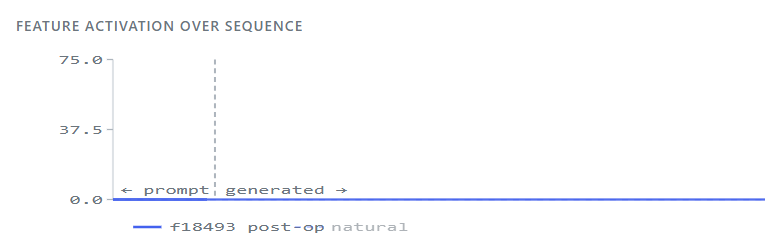
\includegraphics[width=0.85\textwidth]{figures/chart_baseline.png}
\caption{Baseline (flat, no intervention). Feature 18493 activates naturally only on relevant tokens, and as such the stays on-topic with Colorado land animals. }
\end{figure}

\begin{figure}[H]
\centering
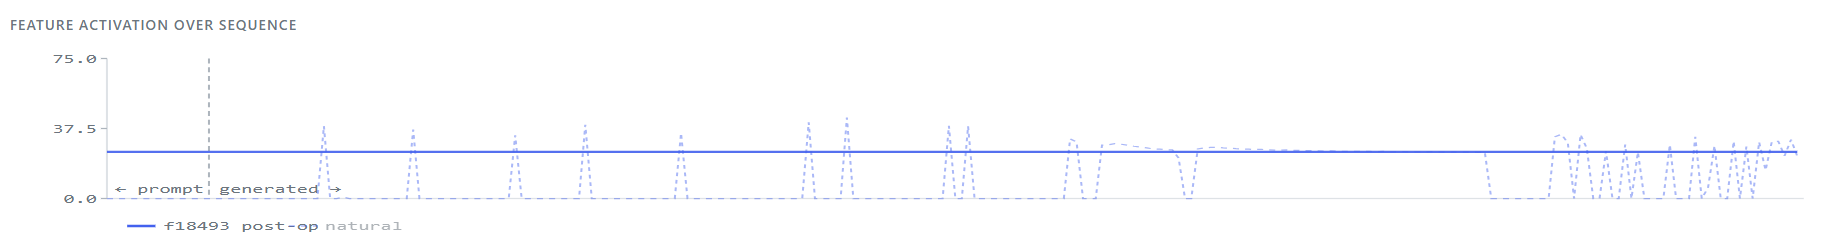
\includegraphics[width=0.85\textwidth]{figures/chart_clamp25.png}
\caption{ClampOp(25). The post-intervention line is flat at 25 across all tokens. Marine content begins to appear but sentence structure is visibly disrupted. Degradation observable in the plot at the end. }
\end{figure}

\begin{figure}[H]
\centering
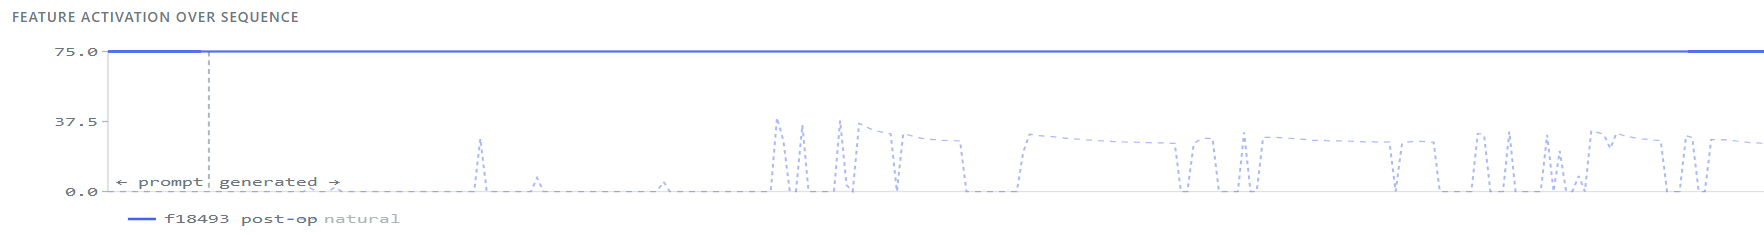
\includegraphics[width=0.85\textwidth]{figures/chart_clamp75.png}
\caption{ClampOp(75). The post-intervention line is flat at 75. The response degrades almost immediately into incoherent marine fragments.}
\end{figure}

\begin{figure}[H]
\centering
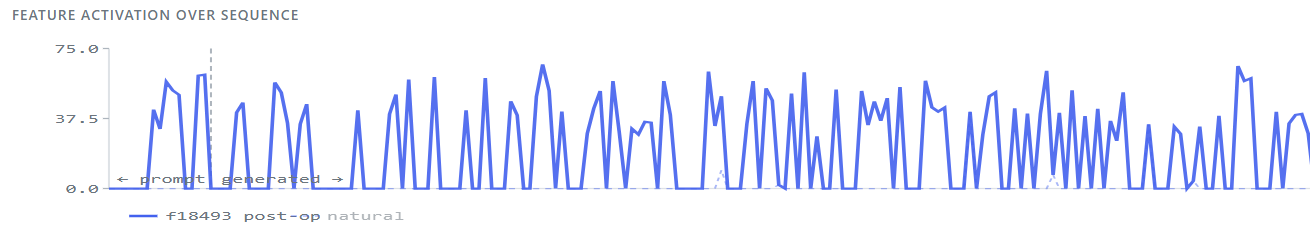
\includegraphics[width=0.85\textwidth]{figures/chart_conddist.png}
\caption{CondDistOp($\mathcal{N}(45,10)$, $p=0.4$). The post-intervention line shows intermittent spikes where the sampler fired; between spikes the model generates naturally. The response is coherent and marine-themed.}
\end{figure}

\subsection{Operation Tuning}

The grid search over the 594 combinations of $p$, $\mu$, and $\sigma$ yields consistent patterns. The dominant finding is that $p$ controls the tradeoff between steering strength and response quality: above roughly $p \approx 0.5$, coherency and relatability degrade sharply regardless of $\mu$ or $\sigma$, while below $p \approx 0.4$ the steering effect becomes inconsistent. $\mu$ raises shark-strength monotonically but has diminishing returns above $\mu = 60$. $\sigma > 0$ modestly improves coherency at the cost of a less consistent steering signal; $\sigma = 10$ appears to be a reasonable compromise.

\begin{figure}[H]
\begin{adjustwidth}{-1.8cm}{-1.4cm}
\centering
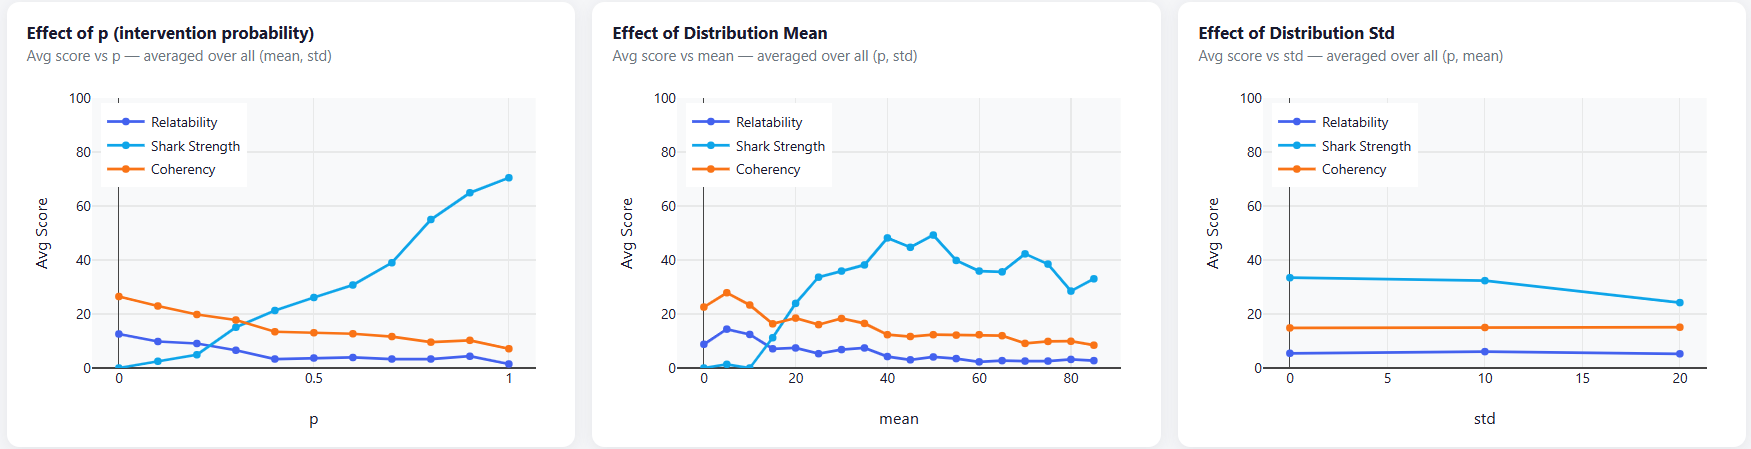
\includegraphics[width=8in]{figures/param_effects.png}
\caption{Effect of $p$, $\mu$, and $\sigma$ on coherency, relatability, and shark-strength.}
\end{adjustwidth}
\end{figure}

\begin{figure}[H]
\centering
\begin{adjustwidth}{-1.8cm}{-1.4cm}
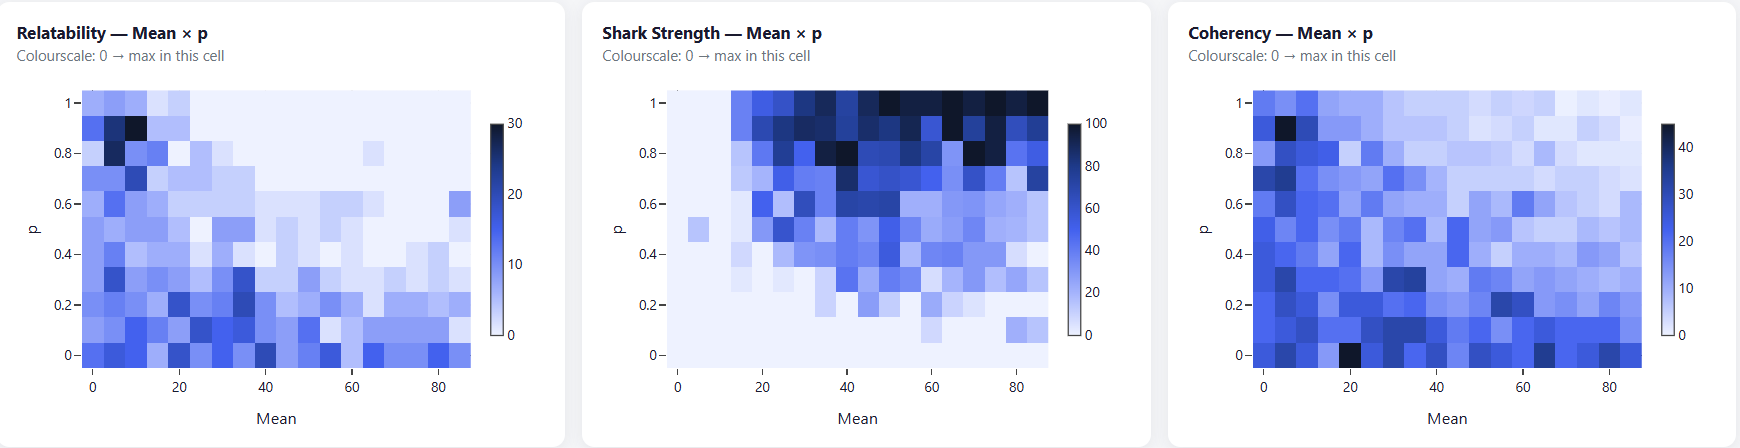
\includegraphics[width=8in]{figures/heatmap.png}
\caption{Shark-strength as a function of $\mu$ (x-axis) and $p$ (y-axis) at $\sigma = 10$. The transition from low to high shark-strength occurs near $p = 0.3$--$0.4$ and $\mu = 40$--$60$.}
\end{adjustwidth}
\end{figure}

\subsection{Signed Activations and Projection Steering}
We combine the results for the trained SAEs and projection steering, as the two are closely related. Shown below is a plot of the loss by training step. It is important to note that the loss landscape changes drastically after the warmup finishes at step 20,000 when sparsity begins to be enforced for Topk, Shrink, and AbsTopK.
\begin{figure}[!h]
    \centering
    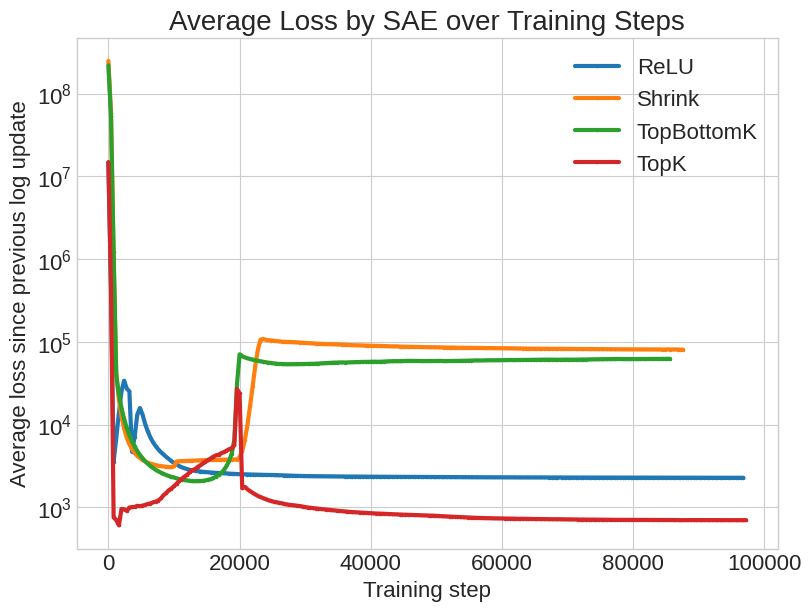
\includegraphics[width=0.5\linewidth]{figures/loss_landscape.png}
    \caption{Plot of average loss by training step for each SAE}
    \label{fig:placeholder}
\end{figure}

We qualitatively compare the different SAEs with their ability to steer via vector addition and projection. Using the methodology described in section 4.5.1, we obtain an average feature vector for the concepts happy, sad, hot, and cold. We then feed a selection of "Sensitive" and "Invariant" prompts - prompts that ideally would change with steering, and ones that should not change with steering. \\See the Appendix for some examples.

\begin{center}
    \textbf{Takeaways from Comparing Different Trained SAEs}
\end{center}
    \begin{enumerate}
        \item We observed that SAEs with negative-valued activations were more resilient to vector additions with large scaling factors (15).
        \item As could be expected, the projection steering didn't perform remotely well on the positive-valued SAEs, but works well with the negative-valued ones.
        \item Compared to the other SAEs, Shrink produced more sensible results for both steering methods.
    \end{enumerate}
\begin{center}
    \textbf{Takeaways from Comparing Different Steering Methods with Shrink Activation }
\end{center}
    Diving into the Shrink SAE performance, we observe the following:
    \begin{enumerate}
        \item Orthogonal subspace projections were more subtle in steering sensitive prompts than vector addition (scaled factor = 15). In other words, projections allowed for effective steering without dominating the sentence with a certain idea.
        \item Both vector addition and projection did not change responses of invariant prompts very much.
        \item Projection steering does not always nudge the sentence in the intended direction - See the "happy" projection of the princess prompt.
    \end{enumerate}


\section{Future Work}

This project was conducted in a fairly short time span. As a result, the primary need for further work is in increased experimentation. A more rigorous testing framework could show how robust these methods are.\\

There are countless other variations upon steering methods that could be proposed, and either a more formal mathematical proposal for which ones will yield desired results, or a larger collection of operations (with equally thorough hyperparameter tunings) that are being evaluated by an LLM (in a similar fashion to the methodology shown here) will go a long way to proving the potential of this fashion of steering.\\

The results demonstrated in regards to inducing biases have only been performed on two fairly simple examples, being positivie/negative attitudes and temperature. A more thorough study into the successes and failures of identifying and steering on these features would be similarly useful, as well as enhancing the complexity of these tasks.

Additionally, SAEs are highly dependent on their training, as is shown in \cite{training}. A more thorough training of professional SAEs using this novel activation function may yield significantly improved results.\\

Finally, all this research was conducted using small local models, compared to the models that are actually deployed in settings where these methods would be useful. As with most all LLMs research, the question of scalability shadows much of this work. While implementing these methods on more sophisticated and larger models would likely make the results of the steering much more clear (due to the more coherent responses), it is not clear if the steering would perform as significantly.

\section{Conclusion}

Overall, the work done for this project shows the significant potential that exists for more advanced and capable model steering that utilizes sparse autoencoders and their unique properties. Key takeaways include:

\begin{enumerate}
    \item \textbf{Model Degradation:} 'Hard clamping' of features results in model degradation, where responses approach steering subject matter as they become useless and repetitive.
    \item \textbf{Stochastic Intervention Methods:} Initial results indicate that alternative methods of intervening on models resolve the model degradation issue and may steer more naturally. Other methods are demonstrated to be viable as well, creating room for further method proposal and development.
    \item \textbf{Hyperparameter Tuning:} We successfully establish methodology for identifying hyperparameters to intervention methods using grid search and a response evaluation pipeline.
    \item \textbf{Proposed feature projection method:} Our proposed method shows promising results in steering responses without degrading the quality.
    \item \textbf{Proposed Shrink Activation Function} works especially well with subspace projection, compared to existing negative-valued activations such as AbsTopK\cite{abstopk}

    \item \textbf{Feature Identification:} We propose, implement, and demonstrate the viability of a workflow for identifying features that may constitute a model bias when combined with the aforementioned steering methods. This may be both a useful tool for steering overall behavior and suggests that SAEs may still be lacking in monosemanticity to a certain extent.
\end{enumerate}

There is much work remaining to be done in this area, but this paper has proposed methods that establish the potential of steering models in this manner.

\bibliographystyle{plain}
\bibliography{refs}
\appendix
\section{Appendix}
Shown below are some steered promp examples, referenced in Section 5.3.

\begin{center}
    \textbf{Sensitive Prompts}
\end{center}\begin{qualbox}{ReLU SAE + Projection Steering}

\textit{Prompt: ``Will I need a blanket today?''}

\vspace{0.4em}

\noindent
\begin{minipage}[t]{0.485\linewidth}
\begin{responsebox}{Baseline}{baselinegray}
\footnotesize
No, you will not need a blanket today.
\end{responsebox}
\end{minipage}
\hfill
\begin{minipage}[t]{0.485\linewidth}
\begin{responsebox}{Cold-Steered}{coldblue}
\footnotesize
``nieve'', hyphenı llegue llegue'', hyphenı llegue
\end{responsebox}
\end{minipage}

\end{qualbox}

\vspace{0.5em}

\begin{qualbox}{TopK SAE + Projection Steering}

\textit{Prompt: ``Will I need a blanket today?''}

\vspace{0.4em}

\noindent
\begin{minipage}[t]{0.485\linewidth}
\begin{responsebox}{Baseline}{baselinegray}
\footnotesize
No, you will not need a blanket today.
\end{responsebox}
\end{minipage}
\hfill
\begin{minipage}[t]{0.485\linewidth}
\begin{responsebox}{Cold-Steered}{coldblue}
\footnotesize
``\#''taaledningthewUNITED ``latego taken taken''
\end{responsebox}
\end{minipage}

\end{qualbox}

\vspace{0.5em}

\begin{qualbox}{Shrink SAE + Projection Steering}

\textit{Prompt: ``Will I need a blanket today?''}

\vspace{0.4em}

\noindent
\begin{minipage}[t]{0.485\linewidth}
\begin{responsebox}{Baseline}{baselinegray}
\footnotesize
No, you will not need a blanket today.
\end{responsebox}
\end{minipage}
\hfill
\begin{minipage}[t]{0.485\linewidth}
\begin{responsebox}{Cold-Steered}{coldblue}
\footnotesize
Yes, you will need a blanket today.
\end{responsebox}
\end{minipage}

\end{qualbox}

\vspace{0.5em}

\begin{qualbox}{AbsTopK SAE + Projection Steering}

\textit{Prompt: ``Will I need a blanket today?''}

\vspace{0.4em}

\noindent
\begin{minipage}[t]{0.485\linewidth}
\begin{responsebox}{Baseline}{baselinegray}
\footnotesize
No, you will not need a blanket today.
\end{responsebox}
\end{minipage}
\hfill
\begin{minipage}[t]{0.485\linewidth}
\begin{responsebox}{Cold-Steered}{coldblue}
\footnotesize
arnyaвой \textbackslash{}érience 아멘\textbackslash{}. practicar 아멘 convenc
\end{responsebox}
\end{minipage}

\end{qualbox}

\begin{center}
    \textbf{Invariant Prompts}
\end{center}


\begin{qualbox}{ReLU SAE + Vector Addition Steering}

\textit{Prompt: ``What is the capital of France?''}

\vspace{0.4em}

\noindent
\begin{minipage}[t]{0.485\linewidth}
\begin{responsebox}{Baseline}{baselinegray}
\footnotesize
The capital of France is Paris.
\end{responsebox}
\end{minipage}
\hfill
\begin{minipage}[t]{0.485\linewidth}
\begin{responsebox}{Cold-Steered}{coldblue}
\footnotesize
``Winter'', as the winter was the only state in the Union''
\end{responsebox}
\end{minipage}

\end{qualbox}

\vspace{0.5em}

\begin{qualbox}{TopK SAE + Vector Addition Steering}

\textit{Prompt: ``What is the capital of France?''}

\vspace{0.4em}

\noindent
\begin{minipage}[t]{0.485\linewidth}
\begin{responsebox}{Baseline}{baselinegray}
\footnotesize
The capital of France is Paris.
\end{responsebox}
\end{minipage}
\hfill
\begin{minipage}[t]{0.485\linewidth}
\begin{responsebox}{Cold-Steered}{coldblue}
\footnotesize
``No Pakistan''ట్టు the benefit la TiPEN DU''
\end{responsebox}
\end{minipage}

\end{qualbox}

\vspace{0.5em}

\begin{qualbox}{Shrink SAE + Vector Addition Steering}

\textit{Prompt: ``What is the capital of France?''}

\vspace{0.4em}

\noindent
\begin{minipage}[t]{0.485\linewidth}
\begin{responsebox}{Baseline}{baselinegray}
\footnotesize
The capital of France is Paris.
\end{responsebox}
\end{minipage}
\hfill
\begin{minipage}[t]{0.485\linewidth}
\begin{responsebox}{Cold-Steered}{coldblue}
\footnotesize
Yes, you will need a blanket today.
\end{responsebox}
\end{minipage}

\end{qualbox}

\vspace{0.5em}

\begin{qualbox}{AbsTopK SAE + Vector Addition Steering}

\textit{Prompt: ``What is the capital of France?''}

\vspace{0.4em}

\noindent
\begin{minipage}[t]{0.485\linewidth}
\begin{responsebox}{Baseline}{baselinegray}
\footnotesize
The capital of France is Paris.
\end{responsebox}
\end{minipage}
\hfill
\begin{minipage}[t]{0.485\linewidth}
\begin{responsebox}{Cold-Steered}{coldblue}
\footnotesize
The capital of France is Paris.
\end{responsebox}
\end{minipage}

\end{qualbox}
\end{document}
